
\section{Results}
\label{sec:results}

     To evaluate our data, we took a subset of the Generator 1 data
and split it into training and test sets. We noticed that the
data varied very little outside the range [-50, 50], so we
considered x-values from [-50,50] in increments of 0.1, and
their corresponding y-values.\\

Our algorithm produced spectacular results, finding an equation for
the Generator 1 data with less than 5 x 10-15 total error on the test
set. When evolving, this tree took 19 generations to be formed. After
19 generations, the equation  $$\frac{10}{x^2-6x+14}$$  had a total error of
less than 2x10-14 when evaluated on the test set, as stated above, the
error was similarly low. This indicates that the equation generalizes
well and was not overfit to the training data.\\

After ten runs of GP, we had ten trees that were each the best in that iteration of the algorithm. On average, one of these winning trees had an error of 31.27 on the test set with a standard deviation of 22.34. When considered in the scope of the size of the test set, these results are quite impressive. An error of 31 means that over the 200 datapoints in the test set, the derived function generated values that were on average 0.15 off from the actual values.\\

\begin{figure}[htb]

  \centering  % centers the image in the column

  % replace the second argument below with your filename. I like to
  % place all my figures in a sub-directory to keep things organized
  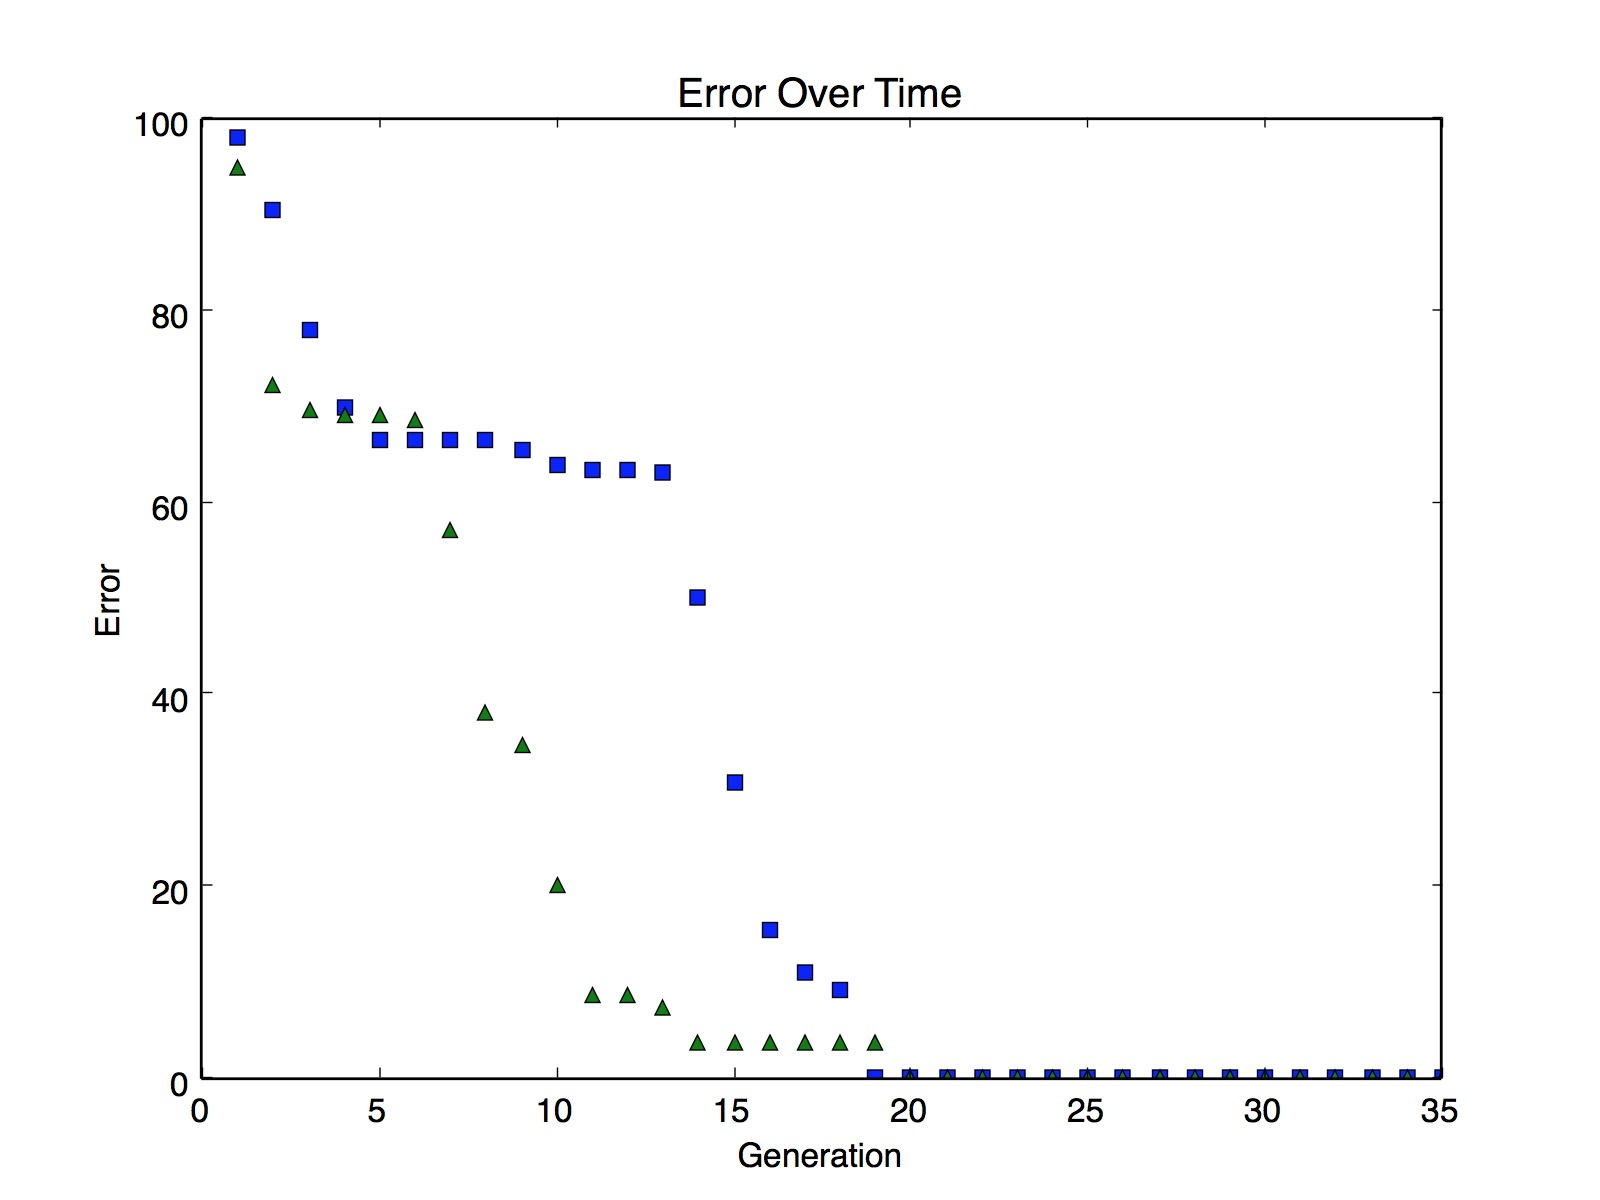
\includegraphics[width=0.5\textwidth]{figs/Generator1.jpg}

  % *Every* figure should have a descriptive caption.
  \caption{This figure depicts the best ablsolute error score for each
    generation of several genetic programming runs. Each of the runs
    depicted were the best runs of a full experimental run of 10 runs of
    genetic programming.}


  \label{fig:tex}

\end{figure}

